\documentclass[twoside]{book}

% Packages required by doxygen
\usepackage{fixltx2e}
\usepackage{calc}
\usepackage{doxygen}
\usepackage[export]{adjustbox} % also loads graphicx
\usepackage{graphicx}
\usepackage[utf8]{inputenc}
\usepackage{makeidx}
\usepackage{multicol}
\usepackage{multirow}
\PassOptionsToPackage{warn}{textcomp}
\usepackage{textcomp}
\usepackage[nointegrals]{wasysym}
\usepackage[table]{xcolor}

% Font selection
\usepackage[T1]{fontenc}
\usepackage[scaled=.90]{helvet}
\usepackage{courier}
\usepackage{amssymb}
\usepackage{sectsty}
\renewcommand{\familydefault}{\sfdefault}
\allsectionsfont{%
  \fontseries{bc}\selectfont%
  \color{darkgray}%
}
\renewcommand{\DoxyLabelFont}{%
  \fontseries{bc}\selectfont%
  \color{darkgray}%
}
\newcommand{\+}{\discretionary{\mbox{\scriptsize$\hookleftarrow$}}{}{}}

% Page & text layout
\usepackage{geometry}
\geometry{%
  a4paper,%
  top=2.5cm,%
  bottom=2.5cm,%
  left=2.5cm,%
  right=2.5cm%
}
\tolerance=750
\hfuzz=15pt
\hbadness=750
\setlength{\emergencystretch}{15pt}
\setlength{\parindent}{0cm}
\setlength{\parskip}{3ex plus 2ex minus 2ex}
\makeatletter
\renewcommand{\paragraph}{%
  \@startsection{paragraph}{4}{0ex}{-1.0ex}{1.0ex}{%
    \normalfont\normalsize\bfseries\SS@parafont%
  }%
}
\renewcommand{\subparagraph}{%
  \@startsection{subparagraph}{5}{0ex}{-1.0ex}{1.0ex}{%
    \normalfont\normalsize\bfseries\SS@subparafont%
  }%
}
\makeatother

% Headers & footers
\usepackage{fancyhdr}
\pagestyle{fancyplain}
\fancyhead[LE]{\fancyplain{}{\bfseries\thepage}}
\fancyhead[CE]{\fancyplain{}{}}
\fancyhead[RE]{\fancyplain{}{\bfseries\leftmark}}
\fancyhead[LO]{\fancyplain{}{\bfseries\rightmark}}
\fancyhead[CO]{\fancyplain{}{}}
\fancyhead[RO]{\fancyplain{}{\bfseries\thepage}}
\fancyfoot[LE]{\fancyplain{}{}}
\fancyfoot[CE]{\fancyplain{}{}}
\fancyfoot[RE]{\fancyplain{}{\bfseries\scriptsize Generated by Doxygen }}
\fancyfoot[LO]{\fancyplain{}{\bfseries\scriptsize Generated by Doxygen }}
\fancyfoot[CO]{\fancyplain{}{}}
\fancyfoot[RO]{\fancyplain{}{}}
\renewcommand{\footrulewidth}{0.4pt}
\renewcommand{\chaptermark}[1]{%
  \markboth{#1}{}%
}
\renewcommand{\sectionmark}[1]{%
  \markright{\thesection\ #1}%
}

% Indices & bibliography
\usepackage{natbib}
\usepackage[titles]{tocloft}
\setcounter{tocdepth}{3}
\setcounter{secnumdepth}{5}
\makeindex

% Hyperlinks (required, but should be loaded last)
\usepackage{ifpdf}
\ifpdf
  \usepackage[pdftex,pagebackref=true]{hyperref}
\else
  \usepackage[ps2pdf,pagebackref=true]{hyperref}
\fi
\hypersetup{%
  colorlinks=true,%
  linkcolor=blue,%
  citecolor=blue,%
  unicode%
}

% Custom commands
\newcommand{\clearemptydoublepage}{%
  \newpage{\pagestyle{empty}\cleardoublepage}%
}

\usepackage{caption}
\captionsetup{labelsep=space,justification=centering,font={bf},singlelinecheck=off,skip=4pt,position=top}

%===== C O N T E N T S =====

\begin{document}

% Titlepage & ToC
\hypersetup{pageanchor=false,
             bookmarksnumbered=true,
             pdfencoding=unicode
            }
\pagenumbering{alph}
\begin{titlepage}
\vspace*{7cm}
\begin{center}%
{\Large T-\/\+Rex Game }\\
\vspace*{1cm}
{\large Generated by Doxygen 1.8.12}\\
\end{center}
\end{titlepage}
\clearemptydoublepage
\pagenumbering{roman}
\tableofcontents
\clearemptydoublepage
\pagenumbering{arabic}
\hypersetup{pageanchor=true}

%--- Begin generated contents ---
\chapter{Hierarchical Index}
\section{Class Hierarchy}
This inheritance list is sorted roughly, but not completely, alphabetically\+:\begin{DoxyCompactList}
\item Mono\+Behaviour\begin{DoxyCompactList}
\item \contentsline{section}{Background}{\pageref{class_background}}{}
\item \contentsline{section}{Camera}{\pageref{class_camera}}{}
\item \contentsline{section}{Game\+Over}{\pageref{class_game_over}}{}
\item \contentsline{section}{Obstacles}{\pageref{class_obstacles}}{}
\item \contentsline{section}{Start}{\pageref{class_start}}{}
\item \contentsline{section}{T\+Rex}{\pageref{class_t_rex}}{}
\end{DoxyCompactList}
\end{DoxyCompactList}

\chapter{Class Index}
\section{Class List}
Here are the classes, structs, unions and interfaces with brief descriptions\+:\begin{DoxyCompactList}
\item\contentsline{section}{\hyperlink{class_background}{Background} }{\pageref{class_background}}{}
\item\contentsline{section}{\hyperlink{class_camera}{Camera} }{\pageref{class_camera}}{}
\item\contentsline{section}{\hyperlink{class_game_over}{Game\+Over} }{\pageref{class_game_over}}{}
\item\contentsline{section}{\hyperlink{class_obstacles}{Obstacles} }{\pageref{class_obstacles}}{}
\item\contentsline{section}{\hyperlink{class_start}{Start} }{\pageref{class_start}}{}
\item\contentsline{section}{\hyperlink{class_t_rex}{T\+Rex} }{\pageref{class_t_rex}}{}
\end{DoxyCompactList}

\chapter{Class Documentation}
\hypertarget{class_background}{}\section{Background Class Reference}
\label{class_background}\index{Background@{Background}}
Inheritance diagram for Background\+:\begin{figure}[H]
\begin{center}
\leavevmode
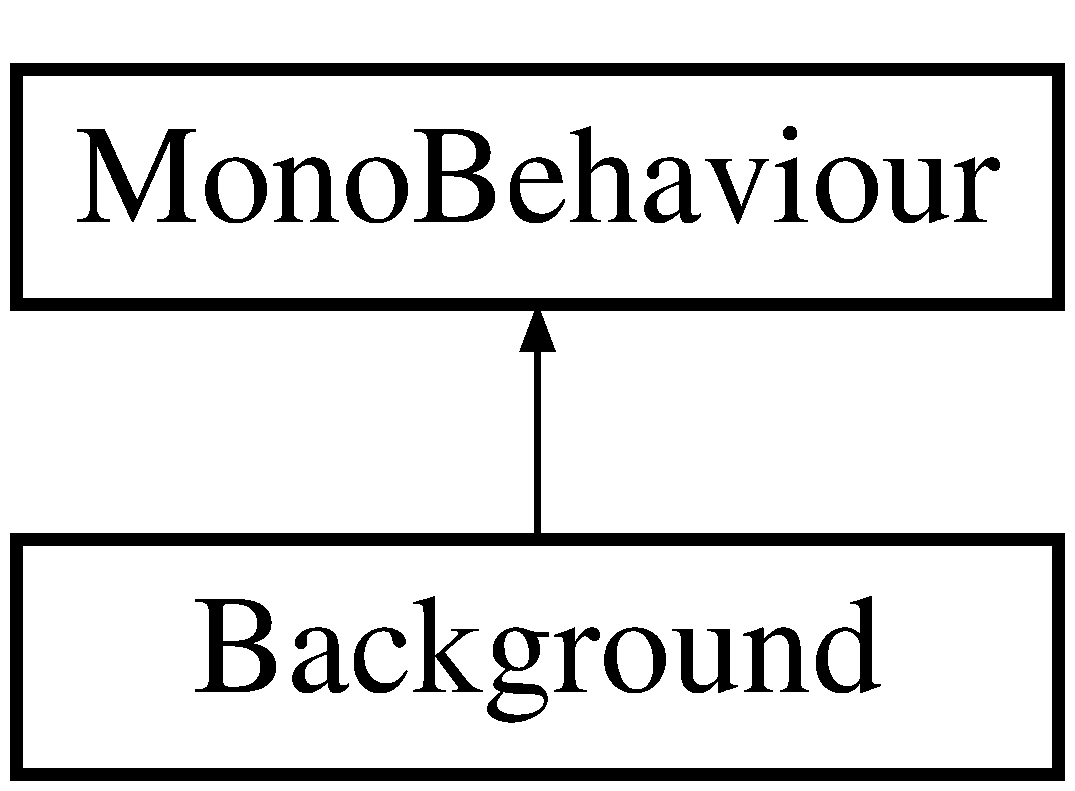
\includegraphics[height=2.000000cm]{class_background}
\end{center}
\end{figure}
\subsection*{Private Member Functions}
\begin{DoxyCompactItemize}
\item 
void \hyperlink{class_background_ab1cd39876241a9c16a96be95d4da8ab8}{On\+Trigger\+Exit2D} (Collider2D collider)
\end{DoxyCompactItemize}


\subsection{Detailed Description}
$<$\+Background$>$ Kelas B\+G\+Shift berfungsi untuk menangani pergerakan background agar background mengeikut pergerakan kamera pada saat game berjalan. $<$/\+Bacground$>$ 

\subsection{Member Function Documentation}
\hypertarget{class_background_ab1cd39876241a9c16a96be95d4da8ab8}{}\label{class_background_ab1cd39876241a9c16a96be95d4da8ab8} 
\index{Background@{Background}!On\+Trigger\+Exit2D@{On\+Trigger\+Exit2D}}
\index{On\+Trigger\+Exit2D@{On\+Trigger\+Exit2D}!Background@{Background}}
\subsubsection{\texorpdfstring{On\+Trigger\+Exit2\+D()}{OnTriggerExit2D()}}
{\footnotesize\ttfamily void Background.\+On\+Trigger\+Exit2D (\begin{DoxyParamCaption}\item[{Collider2D}]{collider }\end{DoxyParamCaption})\hspace{0.3cm}{\ttfamily [private]}}

$<$on\+Trigger\+Exit2\+D$>$ Method ini berfungsi untuk menangani perpihanan background agar mengikuti pergerakan kamera, dengan cara melakukan perturakan background dengan tujuan untuk menghemat penggunaan memori. $<$/on\+Trigger\+Exit2\+D$>$ 

The documentation for this class was generated from the following file\+:\begin{DoxyCompactItemize}
\item 
E\+:/\+Kuliah -\/ temporary/\+Semester 3/\+A\+D\+B\+O/\+Tugas Besar/\+T-\/\+Rex Final/assets/\+Scripts/Background.\+cs\end{DoxyCompactItemize}

\hypertarget{class_camera}{}\section{Camera Class Reference}
\label{class_camera}\index{Camera@{Camera}}
Inheritance diagram for Camera\+:\begin{figure}[H]
\begin{center}
\leavevmode
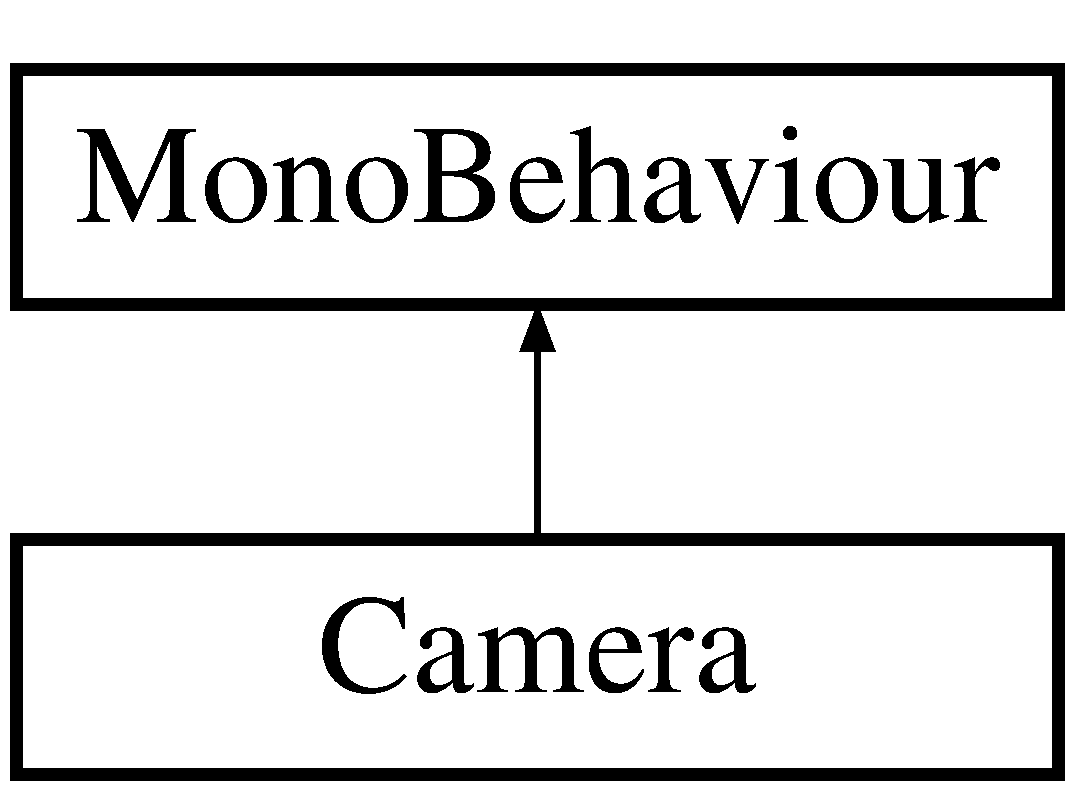
\includegraphics[height=2.000000cm]{class_camera}
\end{center}
\end{figure}
\subsection*{Public Attributes}
\begin{DoxyCompactItemize}
\item 
Transform \hyperlink{class_camera_acfd163e2a143a6b425494de9e86c5e00}{Box}
\item 
G\+U\+I\+Style \hyperlink{class_camera_afaadb7e35bf0918a0abcb53e73a2c565}{style}
\item 
float \hyperlink{class_camera_a8b771a0c2cb6e4fd4b3213a87e0f1a88}{score\+Counter} =0.\+0f
\item 
int \hyperlink{class_camera_abf86e03ac82c531858df39468f8e190b}{score}
\item 
int \hyperlink{class_camera_a91a3b4274da61a63a00782824cf5542e}{high\+Score}
\item 
float \hyperlink{class_camera_a9afbcb25512024bd94c4abc84c85d651}{speed} = 7f
\item 
Audio\+Source \hyperlink{class_camera_a265abd887260923d3b565aed0688cda7}{audi100}
\end{DoxyCompactItemize}
\subsection*{Private Member Functions}
\begin{DoxyCompactItemize}
\item 
void \hyperlink{class_camera_a6dd760883224d50af4d916ca57a26370}{Start} ()
\item 
void \hyperlink{class_camera_a0dd18d8bd55c82e18a9ef12b036eedab}{Update} ()
\item 
void \hyperlink{class_camera_a59fc70f1cd765b02d2858e2fe51d2013}{On\+G\+UI} ()
\item 
void \hyperlink{class_camera_a15e8198aec6c455bfc5016d64152a92c}{Get\+High\+Score} ()
\end{DoxyCompactItemize}


\subsection{Detailed Description}
$<$\+Camera$>$ Kelas Cam\+Runner berfungsi untuk membuat camera bergerak maju secara terus menerus hingga game berakhir. $<$/\+Camera$>$ 

\subsection{Member Function Documentation}
\hypertarget{class_camera_a15e8198aec6c455bfc5016d64152a92c}{}\label{class_camera_a15e8198aec6c455bfc5016d64152a92c} 
\index{Camera@{Camera}!Get\+High\+Score@{Get\+High\+Score}}
\index{Get\+High\+Score@{Get\+High\+Score}!Camera@{Camera}}
\subsubsection{\texorpdfstring{Get\+High\+Score()}{GetHighScore()}}
{\footnotesize\ttfamily void Camera.\+Get\+High\+Score (\begin{DoxyParamCaption}{ }\end{DoxyParamCaption})\hspace{0.3cm}{\ttfamily [private]}}

$<$get\+High\+Score$>$ method untuk menentukan score dan highscore. $<$/get\+High\+Score$>$ \hypertarget{class_camera_a59fc70f1cd765b02d2858e2fe51d2013}{}\label{class_camera_a59fc70f1cd765b02d2858e2fe51d2013} 
\index{Camera@{Camera}!On\+G\+UI@{On\+G\+UI}}
\index{On\+G\+UI@{On\+G\+UI}!Camera@{Camera}}
\subsubsection{\texorpdfstring{On\+G\+U\+I()}{OnGUI()}}
{\footnotesize\ttfamily void Camera.\+On\+G\+UI (\begin{DoxyParamCaption}{ }\end{DoxyParamCaption})\hspace{0.3cm}{\ttfamily [private]}}

$<$on\+G\+U\+I$>$ Method yang berfungsi untuk mengeluarkan highscore dan score ke layar. $<$/on\+G\+U\+I$>$ \hypertarget{class_camera_a6dd760883224d50af4d916ca57a26370}{}\label{class_camera_a6dd760883224d50af4d916ca57a26370} 
\index{Camera@{Camera}!Start@{Start}}
\index{Start@{Start}!Camera@{Camera}}
\subsubsection{\texorpdfstring{Start()}{Start()}}
{\footnotesize\ttfamily void Camera.\+Start (\begin{DoxyParamCaption}{ }\end{DoxyParamCaption})\hspace{0.3cm}{\ttfamily [private]}}

$<$\+Start$>$ Method start berfungsi untuk melakukan inisialisasi pertama pada saat kelas ini dipanggil. $<$/\+Start$>$ \hypertarget{class_camera_a0dd18d8bd55c82e18a9ef12b036eedab}{}\label{class_camera_a0dd18d8bd55c82e18a9ef12b036eedab} 
\index{Camera@{Camera}!Update@{Update}}
\index{Update@{Update}!Camera@{Camera}}
\subsubsection{\texorpdfstring{Update()}{Update()}}
{\footnotesize\ttfamily void Camera.\+Update (\begin{DoxyParamCaption}{ }\end{DoxyParamCaption})\hspace{0.3cm}{\ttfamily [private]}}

$<$\+Update$>$ Method update berfungsi untuk menangani kasus-\/kasus disaat terjadi perubahan frame pada saat game sedang berjalan. $<$/\+Update$>$ 

\subsection{Member Data Documentation}
\hypertarget{class_camera_a265abd887260923d3b565aed0688cda7}{}\label{class_camera_a265abd887260923d3b565aed0688cda7} 
\index{Camera@{Camera}!audi100@{audi100}}
\index{audi100@{audi100}!Camera@{Camera}}
\subsubsection{\texorpdfstring{audi100}{audi100}}
{\footnotesize\ttfamily Audio\+Source Camera.\+audi100}

$<$audi100$>$ Attribute audi100 berfungsi untuk menyimpan suara. $<$/audi100$>$ \hypertarget{class_camera_acfd163e2a143a6b425494de9e86c5e00}{}\label{class_camera_acfd163e2a143a6b425494de9e86c5e00} 
\index{Camera@{Camera}!Box@{Box}}
\index{Box@{Box}!Camera@{Camera}}
\subsubsection{\texorpdfstring{Box}{Box}}
{\footnotesize\ttfamily Transform Camera.\+Box}

$<$\+Box$>$ Attribute yang berfungsi untuk menyimpan nilai box. $<$/\+Box$>$ \hypertarget{class_camera_a91a3b4274da61a63a00782824cf5542e}{}\label{class_camera_a91a3b4274da61a63a00782824cf5542e} 
\index{Camera@{Camera}!high\+Score@{high\+Score}}
\index{high\+Score@{high\+Score}!Camera@{Camera}}
\subsubsection{\texorpdfstring{high\+Score}{highScore}}
{\footnotesize\ttfamily int Camera.\+high\+Score}

$<$high\+Score$>$ Attribute hi berfungsi untuk menyimpan score tertinggi. $<$/high\+Score$>$ \hypertarget{class_camera_abf86e03ac82c531858df39468f8e190b}{}\label{class_camera_abf86e03ac82c531858df39468f8e190b} 
\index{Camera@{Camera}!score@{score}}
\index{score@{score}!Camera@{Camera}}
\subsubsection{\texorpdfstring{score}{score}}
{\footnotesize\ttfamily int Camera.\+score}

$<$score$>$ Attribute score berfungsi untuk menyimpan score pemain. $<$/score$>$ \hypertarget{class_camera_a8b771a0c2cb6e4fd4b3213a87e0f1a88}{}\label{class_camera_a8b771a0c2cb6e4fd4b3213a87e0f1a88} 
\index{Camera@{Camera}!score\+Counter@{score\+Counter}}
\index{score\+Counter@{score\+Counter}!Camera@{Camera}}
\subsubsection{\texorpdfstring{score\+Counter}{scoreCounter}}
{\footnotesize\ttfamily float Camera.\+score\+Counter =0.\+0f}

$<$score\+Counter$>$ Attribute score\+Counter berfungsi untuk menaikan score pemain seiring dengan pergerakan \hyperlink{class_t_rex}{T\+Rex} $<$/score\+Counter$>$ \hypertarget{class_camera_a9afbcb25512024bd94c4abc84c85d651}{}\label{class_camera_a9afbcb25512024bd94c4abc84c85d651} 
\index{Camera@{Camera}!speed@{speed}}
\index{speed@{speed}!Camera@{Camera}}
\subsubsection{\texorpdfstring{speed}{speed}}
{\footnotesize\ttfamily float Camera.\+speed = 7f}





\hypertarget{class_camera_afaadb7e35bf0918a0abcb53e73a2c565}{}\label{class_camera_afaadb7e35bf0918a0abcb53e73a2c565} 
\index{Camera@{Camera}!style@{style}}
\index{style@{style}!Camera@{Camera}}
\subsubsection{\texorpdfstring{style}{style}}
{\footnotesize\ttfamily G\+U\+I\+Style Camera.\+style}

$<$style$>$ Attribute yang berfungsi untuk menangani G\+UI $<$/style$>$ 

The documentation for this class was generated from the following file\+:\begin{DoxyCompactItemize}
\item 
E\+:/\+Kuliah -\/ temporary/\+Semester 3/\+A\+D\+B\+O/\+Tugas Besar/\+T-\/\+Rex Final/assets/\+Scripts/Camera.\+cs\end{DoxyCompactItemize}

\hypertarget{class_game_over}{}\section{Game\+Over Class Reference}
\label{class_game_over}\index{Game\+Over@{Game\+Over}}
Inheritance diagram for Game\+Over\+:\begin{figure}[H]
\begin{center}
\leavevmode
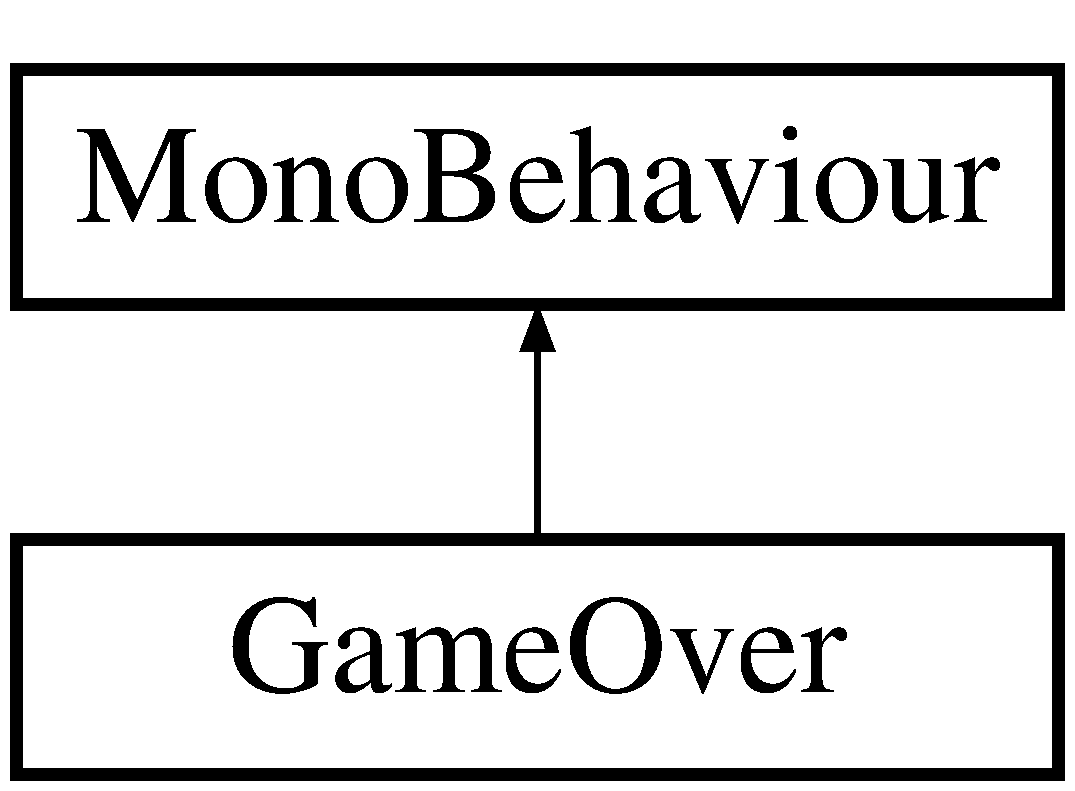
\includegraphics[height=2.000000cm]{class_game_over}
\end{center}
\end{figure}
\subsection*{Public Attributes}
\begin{DoxyCompactItemize}
\item 
bool \hyperlink{class_game_over_a017e52022fa05909ffff9f41cf66556f}{game\+Over}
\item 
\hyperlink{class_start}{Start} \hyperlink{class_game_over_a02e1491bad9373330f05c667aa6eca9d}{ob}
\item 
G\+U\+I\+Style \hyperlink{class_game_over_a038383b18f14cf294618f4f66f919a1d}{style\+Screen}
\item 
Texture \hyperlink{class_game_over_a3d0b130d2f0adc32fad8c776512c4d81}{image1}
\item 
Audio\+Source \mbox{[}$\,$\mbox{]} \hyperlink{class_game_over_a7fc748e99982365f5d3aa91ee48fcaae}{audi\+Over}
\end{DoxyCompactItemize}
\subsection*{Private Member Functions}
\begin{DoxyCompactItemize}
\item 
void \hyperlink{class_game_over_a568be230765aad02fc07c3ff2d655e41}{Start} ()
\begin{DoxyCompactList}\small\item\em Method start berfungsi untuk melakukan inisialisasi pertama pada saat game dimulai. \end{DoxyCompactList}\item 
void \hyperlink{class_game_over_a8da95bbe7fc4559116c077698378bbfb}{On\+Trigger\+Enter2D} (Collider2D collider)
\begin{DoxyCompactList}\small\item\em Method yang berfungsi untuk menangani kasus dimana \hyperlink{class_t_rex}{T\+Rex} menabrak obstacle. \end{DoxyCompactList}\item 
void \hyperlink{class_game_over_abc4992fdbb9d7c3c8134ff24d1944171}{On\+G\+UI} ()
\end{DoxyCompactItemize}


\subsection{Detailed Description}
$<$\+Game\+Over$>$ Kelas yang berfungsi untuk menangani kasus saat game berakhir. $<$/\+Game\+Over$>$ 

\subsection{Member Function Documentation}
\hypertarget{class_game_over_abc4992fdbb9d7c3c8134ff24d1944171}{}\label{class_game_over_abc4992fdbb9d7c3c8134ff24d1944171} 
\index{Game\+Over@{Game\+Over}!On\+G\+UI@{On\+G\+UI}}
\index{On\+G\+UI@{On\+G\+UI}!Game\+Over@{Game\+Over}}
\subsubsection{\texorpdfstring{On\+G\+U\+I()}{OnGUI()}}
{\footnotesize\ttfamily void Game\+Over.\+On\+G\+UI (\begin{DoxyParamCaption}{ }\end{DoxyParamCaption})\hspace{0.3cm}{\ttfamily [private]}}

$<$\+On\+G\+U\+I$>$ Method yang berfungsi untuk menampilkan score ke layar. $<$/\+On\+G\+U\+I$>$ \hypertarget{class_game_over_a8da95bbe7fc4559116c077698378bbfb}{}\label{class_game_over_a8da95bbe7fc4559116c077698378bbfb} 
\index{Game\+Over@{Game\+Over}!On\+Trigger\+Enter2D@{On\+Trigger\+Enter2D}}
\index{On\+Trigger\+Enter2D@{On\+Trigger\+Enter2D}!Game\+Over@{Game\+Over}}
\subsubsection{\texorpdfstring{On\+Trigger\+Enter2\+D()}{OnTriggerEnter2D()}}
{\footnotesize\ttfamily void Game\+Over.\+On\+Trigger\+Enter2D (\begin{DoxyParamCaption}\item[{Collider2D}]{collider }\end{DoxyParamCaption})\hspace{0.3cm}{\ttfamily [private]}}



Method yang berfungsi untuk menangani kasus dimana \hyperlink{class_t_rex}{T\+Rex} menabrak obstacle. 

\hypertarget{class_game_over_a568be230765aad02fc07c3ff2d655e41}{}\label{class_game_over_a568be230765aad02fc07c3ff2d655e41} 
\index{Game\+Over@{Game\+Over}!Start@{Start}}
\index{Start@{Start}!Game\+Over@{Game\+Over}}
\subsubsection{\texorpdfstring{Start()}{Start()}}
{\footnotesize\ttfamily void Game\+Over.\+Start (\begin{DoxyParamCaption}{ }\end{DoxyParamCaption})\hspace{0.3cm}{\ttfamily [private]}}



Method start berfungsi untuk melakukan inisialisasi pertama pada saat game dimulai. 



\subsection{Member Data Documentation}
\hypertarget{class_game_over_a7fc748e99982365f5d3aa91ee48fcaae}{}\label{class_game_over_a7fc748e99982365f5d3aa91ee48fcaae} 
\index{Game\+Over@{Game\+Over}!audi\+Over@{audi\+Over}}
\index{audi\+Over@{audi\+Over}!Game\+Over@{Game\+Over}}
\subsubsection{\texorpdfstring{audi\+Over}{audiOver}}
{\footnotesize\ttfamily Audio\+Source \mbox{[}$\,$\mbox{]} Game\+Over.\+audi\+Over}

$<$audi\+Over$>$ Attribute yang berfungsi untuk menyimpan suara. $<$/audi\+Over$>$ \hypertarget{class_game_over_a017e52022fa05909ffff9f41cf66556f}{}\label{class_game_over_a017e52022fa05909ffff9f41cf66556f} 
\index{Game\+Over@{Game\+Over}!game\+Over@{game\+Over}}
\index{game\+Over@{game\+Over}!Game\+Over@{Game\+Over}}
\subsubsection{\texorpdfstring{game\+Over}{gameOver}}
{\footnotesize\ttfamily bool Game\+Over.\+game\+Over}

$<$game\+Over$>$ Attribute yang menangani jika \hyperlink{class_t_rex}{T\+Rex} telah melewati obstacle. $<$/game\+Over$>$ \hypertarget{class_game_over_a3d0b130d2f0adc32fad8c776512c4d81}{}\label{class_game_over_a3d0b130d2f0adc32fad8c776512c4d81} 
\index{Game\+Over@{Game\+Over}!image1@{image1}}
\index{image1@{image1}!Game\+Over@{Game\+Over}}
\subsubsection{\texorpdfstring{image1}{image1}}
{\footnotesize\ttfamily Texture Game\+Over.\+image1}

$<$image1$>$ Attribute yang berfungsi untuk menyimpan gambar. $<$/image1$>$ \hypertarget{class_game_over_a02e1491bad9373330f05c667aa6eca9d}{}\label{class_game_over_a02e1491bad9373330f05c667aa6eca9d} 
\index{Game\+Over@{Game\+Over}!ob@{ob}}
\index{ob@{ob}!Game\+Over@{Game\+Over}}
\subsubsection{\texorpdfstring{ob}{ob}}
{\footnotesize\ttfamily \hyperlink{class_start}{Start} Game\+Over.\+ob}

$<$ob$>$ Attribute yang menangani $<$/ob$>$ \hypertarget{class_game_over_a038383b18f14cf294618f4f66f919a1d}{}\label{class_game_over_a038383b18f14cf294618f4f66f919a1d} 
\index{Game\+Over@{Game\+Over}!style\+Screen@{style\+Screen}}
\index{style\+Screen@{style\+Screen}!Game\+Over@{Game\+Over}}
\subsubsection{\texorpdfstring{style\+Screen}{styleScreen}}
{\footnotesize\ttfamily G\+U\+I\+Style Game\+Over.\+style\+Screen}

$<$style\+Screen$>$ Attribute yang berfungsi untuk menangai style gambar. $<$/style\+Screen$>$ 

The documentation for this class was generated from the following file\+:\begin{DoxyCompactItemize}
\item 
E\+:/\+Kuliah -\/ temporary/\+Semester 3/\+A\+D\+B\+O/\+Tugas Besar/\+T-\/\+Rex Final/assets/\+Scripts/Game\+Over.\+cs\end{DoxyCompactItemize}

\hypertarget{class_obstacles}{}\section{Obstacles Class Reference}
\label{class_obstacles}\index{Obstacles@{Obstacles}}
Inheritance diagram for Obstacles\+:\begin{figure}[H]
\begin{center}
\leavevmode
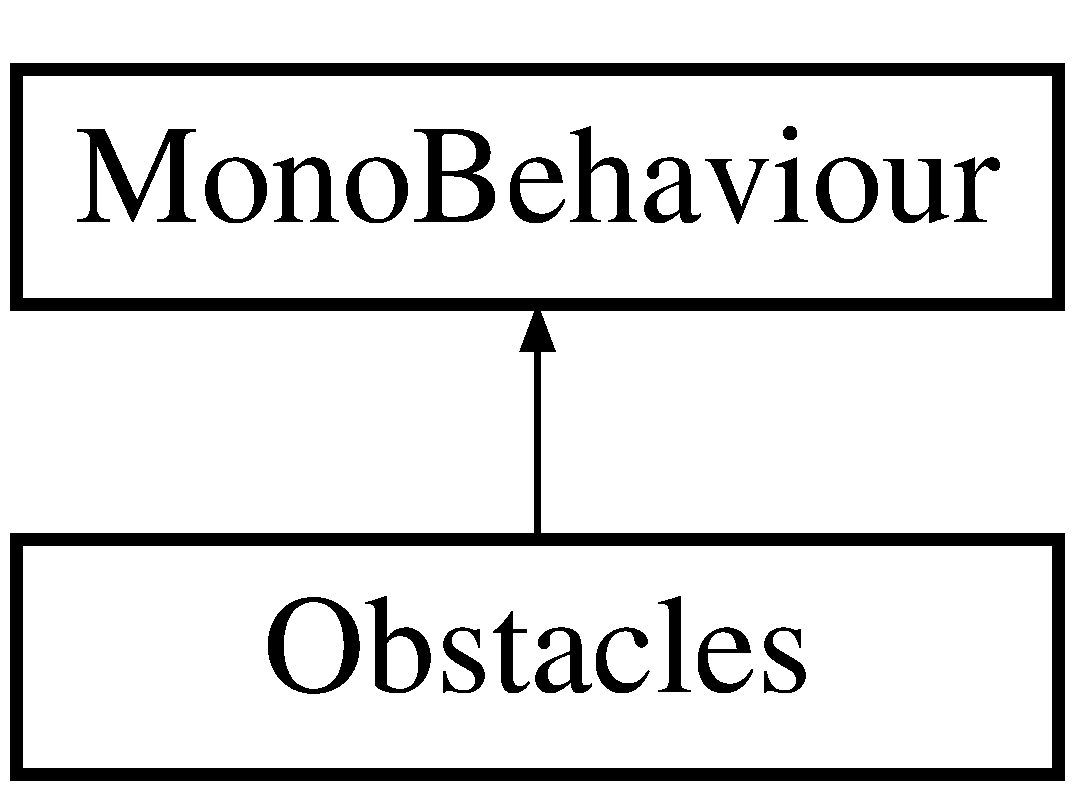
\includegraphics[height=2.000000cm]{class_obstacles}
\end{center}
\end{figure}
\subsection*{Public Attributes}
\begin{DoxyCompactItemize}
\item 
Game\+Object \mbox{[}$\,$\mbox{]} \hyperlink{class_obstacles_af33a9b1d17f969192cf1c0c5357827c9}{challenge}
\item 
Transform \hyperlink{class_obstacles_ad66e2e7a0d3fbd65343001ad795f8625}{campos}
\item 
\hyperlink{class_camera}{Camera} \hyperlink{class_obstacles_aedd2984958638233b3dcc79fe81b0c29}{cam}
\end{DoxyCompactItemize}
\subsection*{Private Member Functions}
\begin{DoxyCompactItemize}
\item 
void \hyperlink{class_obstacles_a32cfaa5f6c916ff526398a7a42dc8928}{Start} ()
\item 
void \hyperlink{class_obstacles_a1c654788f161aa4b2057201f35b41b9b}{Update} ()
\item 
void \hyperlink{class_obstacles_adabe54fa108d13e6200892eb8019a126}{Destroy\+Obstacle} ()
\item 
void \hyperlink{class_obstacles_aa7b4a059d29fce38f79a38e735621698}{Obstacle\+Maker} ()
\end{DoxyCompactItemize}


\subsection{Detailed Description}
$<$\+Obstacles$>$ Kelas ini merupakan kelas untuk membangkitkan obstacle dan pterodactyl dalam permainan T-\/\+Rex Runner. $<$/\+Obstacle$>$ 

\subsection{Member Function Documentation}
\hypertarget{class_obstacles_adabe54fa108d13e6200892eb8019a126}{}\label{class_obstacles_adabe54fa108d13e6200892eb8019a126} 
\index{Obstacles@{Obstacles}!Destroy\+Obstacle@{Destroy\+Obstacle}}
\index{Destroy\+Obstacle@{Destroy\+Obstacle}!Obstacles@{Obstacles}}
\subsubsection{\texorpdfstring{Destroy\+Obstacle()}{DestroyObstacle()}}
{\footnotesize\ttfamily void Obstacles.\+Destroy\+Obstacle (\begin{DoxyParamCaption}{ }\end{DoxyParamCaption})\hspace{0.3cm}{\ttfamily [private]}}

$<$\+Destroy\+Obstacle$>$ method untuk menghancurkan obstacle yang sudah dilewati agar tidak memakan banyak memori. $<$/\+Destroy\+Obstacle$>$ \hypertarget{class_obstacles_aa7b4a059d29fce38f79a38e735621698}{}\label{class_obstacles_aa7b4a059d29fce38f79a38e735621698} 
\index{Obstacles@{Obstacles}!Obstacle\+Maker@{Obstacle\+Maker}}
\index{Obstacle\+Maker@{Obstacle\+Maker}!Obstacles@{Obstacles}}
\subsubsection{\texorpdfstring{Obstacle\+Maker()}{ObstacleMaker()}}
{\footnotesize\ttfamily void Obstacles.\+Obstacle\+Maker (\begin{DoxyParamCaption}{ }\end{DoxyParamCaption})\hspace{0.3cm}{\ttfamily [private]}}

$<$\+Obstacle\+Maker$>$ Method untuk membuat obstacle untuk dilewati T-\/rex. $<$/\+Obstacle\+Maker$>$ \hypertarget{class_obstacles_a32cfaa5f6c916ff526398a7a42dc8928}{}\label{class_obstacles_a32cfaa5f6c916ff526398a7a42dc8928} 
\index{Obstacles@{Obstacles}!Start@{Start}}
\index{Start@{Start}!Obstacles@{Obstacles}}
\subsubsection{\texorpdfstring{Start()}{Start()}}
{\footnotesize\ttfamily void Obstacles.\+Start (\begin{DoxyParamCaption}{ }\end{DoxyParamCaption})\hspace{0.3cm}{\ttfamily [private]}}

$<$\+Start$>$ Method start berfungsi untuk melakukan inisialisasi pertama pada saat kelas ini dipanggil. $<$/\+Start$>$ \hypertarget{class_obstacles_a1c654788f161aa4b2057201f35b41b9b}{}\label{class_obstacles_a1c654788f161aa4b2057201f35b41b9b} 
\index{Obstacles@{Obstacles}!Update@{Update}}
\index{Update@{Update}!Obstacles@{Obstacles}}
\subsubsection{\texorpdfstring{Update()}{Update()}}
{\footnotesize\ttfamily void Obstacles.\+Update (\begin{DoxyParamCaption}{ }\end{DoxyParamCaption})\hspace{0.3cm}{\ttfamily [private]}}

$<$\+Update$>$ Method update berfungsi untuk menangani kasus-\/kasus disaat terjadi perubahan frame pada saat game sedang berjalan. $<$/\+Update$>$ 

\subsection{Member Data Documentation}
\hypertarget{class_obstacles_aedd2984958638233b3dcc79fe81b0c29}{}\label{class_obstacles_aedd2984958638233b3dcc79fe81b0c29} 
\index{Obstacles@{Obstacles}!cam@{cam}}
\index{cam@{cam}!Obstacles@{Obstacles}}
\subsubsection{\texorpdfstring{cam}{cam}}
{\footnotesize\ttfamily \hyperlink{class_camera}{Camera} Obstacles.\+cam}

$<$cam$>$ Attribute yang berfungsi sebagai kamera. $<$/cam$>$ \hypertarget{class_obstacles_ad66e2e7a0d3fbd65343001ad795f8625}{}\label{class_obstacles_ad66e2e7a0d3fbd65343001ad795f8625} 
\index{Obstacles@{Obstacles}!campos@{campos}}
\index{campos@{campos}!Obstacles@{Obstacles}}
\subsubsection{\texorpdfstring{campos}{campos}}
{\footnotesize\ttfamily Transform Obstacles.\+campos}

$<$campos$>$ Attribute yang berfungsi untuk memberitahu posisi dari kamera $<$/campos$>$ \hypertarget{class_obstacles_af33a9b1d17f969192cf1c0c5357827c9}{}\label{class_obstacles_af33a9b1d17f969192cf1c0c5357827c9} 
\index{Obstacles@{Obstacles}!challenge@{challenge}}
\index{challenge@{challenge}!Obstacles@{Obstacles}}
\subsubsection{\texorpdfstring{challenge}{challenge}}
{\footnotesize\ttfamily Game\+Object \mbox{[}$\,$\mbox{]} Obstacles.\+challenge}

$<$challenge$>$ atribut obstacle dari T-\/rex game berupa pohon-\/pohon yang disimpan dalam bentuk array. $<$/challenge$>$ 

The documentation for this class was generated from the following file\+:\begin{DoxyCompactItemize}
\item 
E\+:/\+Kuliah -\/ temporary/\+Semester 3/\+A\+D\+B\+O/\+Tugas Besar/\+T-\/\+Rex Final/assets/\+Scripts/Obstacles.\+cs\end{DoxyCompactItemize}

\hypertarget{class_start}{}\section{Start Class Reference}
\label{class_start}\index{Start@{Start}}
Inheritance diagram for Start\+:\begin{figure}[H]
\begin{center}
\leavevmode
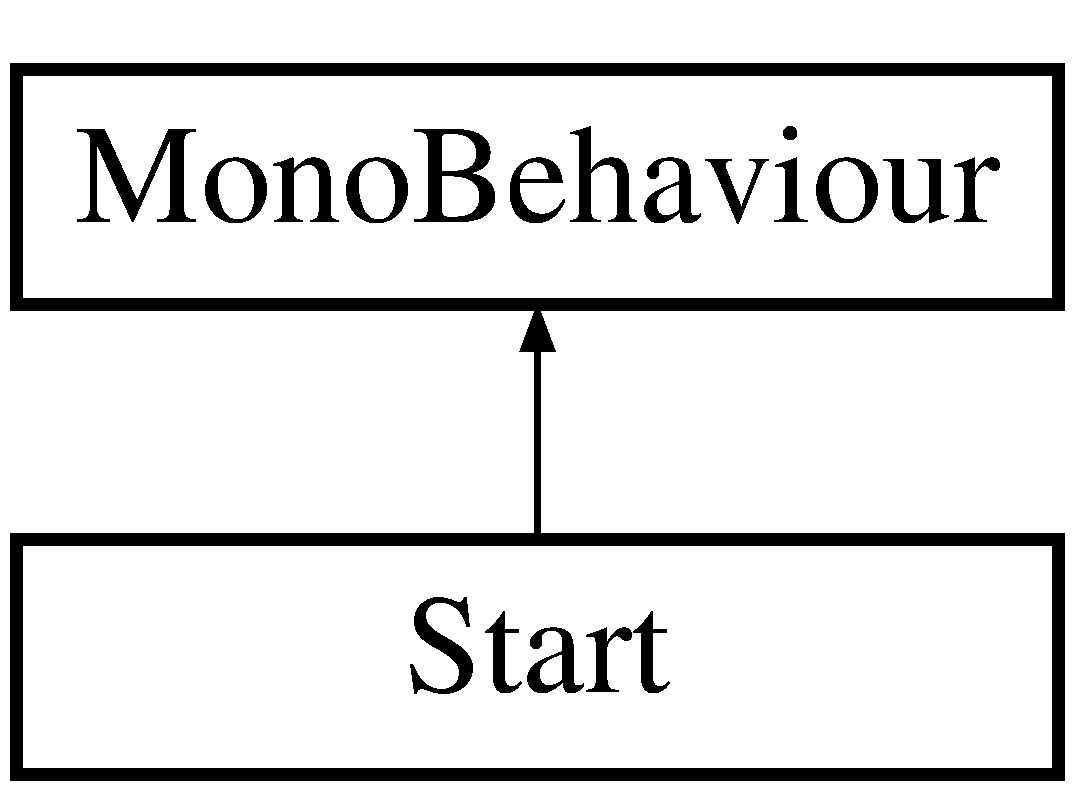
\includegraphics[height=2.000000cm]{class_start}
\end{center}
\end{figure}
\subsection*{Public Attributes}
\begin{DoxyCompactItemize}
\item 
bool \hyperlink{class_start_a3e014e9f3fcc60afaf93ce46b4f23377}{start}
\end{DoxyCompactItemize}
\subsection*{Private Member Functions}
\begin{DoxyCompactItemize}
\item 
void \hyperlink{class_start_ab231df0dc7e25b0bed5c00fd004b99d1}{Awake} ()
\item 
void \hyperlink{class_start_a7911d6483c913d209dda8b107285a721}{Update} ()
\item 
void \hyperlink{class_start_aa9c0928bb57e1ce99c81cc9ad0ab3355}{create\+New\+Game} ()
\end{DoxyCompactItemize}


\subsection{Detailed Description}
$<$\+Start$>$ Kelas yang berfungsi untuk menangani game dimulai pertamakali dan game dimulai setelah gameover / restart game. $<$/\+Start$>$ 

\subsection{Member Function Documentation}
\hypertarget{class_start_ab231df0dc7e25b0bed5c00fd004b99d1}{}\label{class_start_ab231df0dc7e25b0bed5c00fd004b99d1} 
\index{Start@{Start}!Awake@{Awake}}
\index{Awake@{Awake}!Start@{Start}}
\subsubsection{\texorpdfstring{Awake()}{Awake()}}
{\footnotesize\ttfamily void Start.\+Awake (\begin{DoxyParamCaption}{ }\end{DoxyParamCaption})\hspace{0.3cm}{\ttfamily [private]}}

$<$\+Awake$>$ Method yang berfungsi untuk membuat game dapat berjalan kembali. $<$/\+Awake$>$ \hypertarget{class_start_aa9c0928bb57e1ce99c81cc9ad0ab3355}{}\label{class_start_aa9c0928bb57e1ce99c81cc9ad0ab3355} 
\index{Start@{Start}!create\+New\+Game@{create\+New\+Game}}
\index{create\+New\+Game@{create\+New\+Game}!Start@{Start}}
\subsubsection{\texorpdfstring{create\+New\+Game()}{createNewGame()}}
{\footnotesize\ttfamily void Start.\+create\+New\+Game (\begin{DoxyParamCaption}{ }\end{DoxyParamCaption})\hspace{0.3cm}{\ttfamily [private]}}

$<$create\+New\+Game$>$ Method yang berfungsi untuk menangi game yang dimulai kembali saat \hyperlink{class_t_rex}{T\+Rex} telah menabrak obstacle dan game over. $<$/create\+New\+Game$>$ \hypertarget{class_start_a7911d6483c913d209dda8b107285a721}{}\label{class_start_a7911d6483c913d209dda8b107285a721} 
\index{Start@{Start}!Update@{Update}}
\index{Update@{Update}!Start@{Start}}
\subsubsection{\texorpdfstring{Update()}{Update()}}
{\footnotesize\ttfamily void Start.\+Update (\begin{DoxyParamCaption}{ }\end{DoxyParamCaption})\hspace{0.3cm}{\ttfamily [private]}}

$<$\+Update$>$ Method update berfungsi untuk menangani kasus-\/kasus disaat terjadi perubahan frame pada saat game sedang berjalan. $<$/\+Update$>$ 

\subsection{Member Data Documentation}
\hypertarget{class_start_a3e014e9f3fcc60afaf93ce46b4f23377}{}\label{class_start_a3e014e9f3fcc60afaf93ce46b4f23377} 
\index{Start@{Start}!start@{start}}
\index{start@{start}!Start@{Start}}
\subsubsection{\texorpdfstring{start}{start}}
{\footnotesize\ttfamily bool Start.\+start}

$<$start$>$ Attribute yang berfungsi untuk mengetahui apakah game sedang berjalan atau tidak. $<$/start$>$ 

The documentation for this class was generated from the following file\+:\begin{DoxyCompactItemize}
\item 
E\+:/\+Kuliah -\/ temporary/\+Semester 3/\+A\+D\+B\+O/\+Tugas Besar/\+T-\/\+Rex Final/assets/\+Scripts/Start.\+cs\end{DoxyCompactItemize}

\hypertarget{class_t_rex}{}\section{T\+Rex Class Reference}
\label{class_t_rex}\index{T\+Rex@{T\+Rex}}
Inheritance diagram for T\+Rex\+:\begin{figure}[H]
\begin{center}
\leavevmode
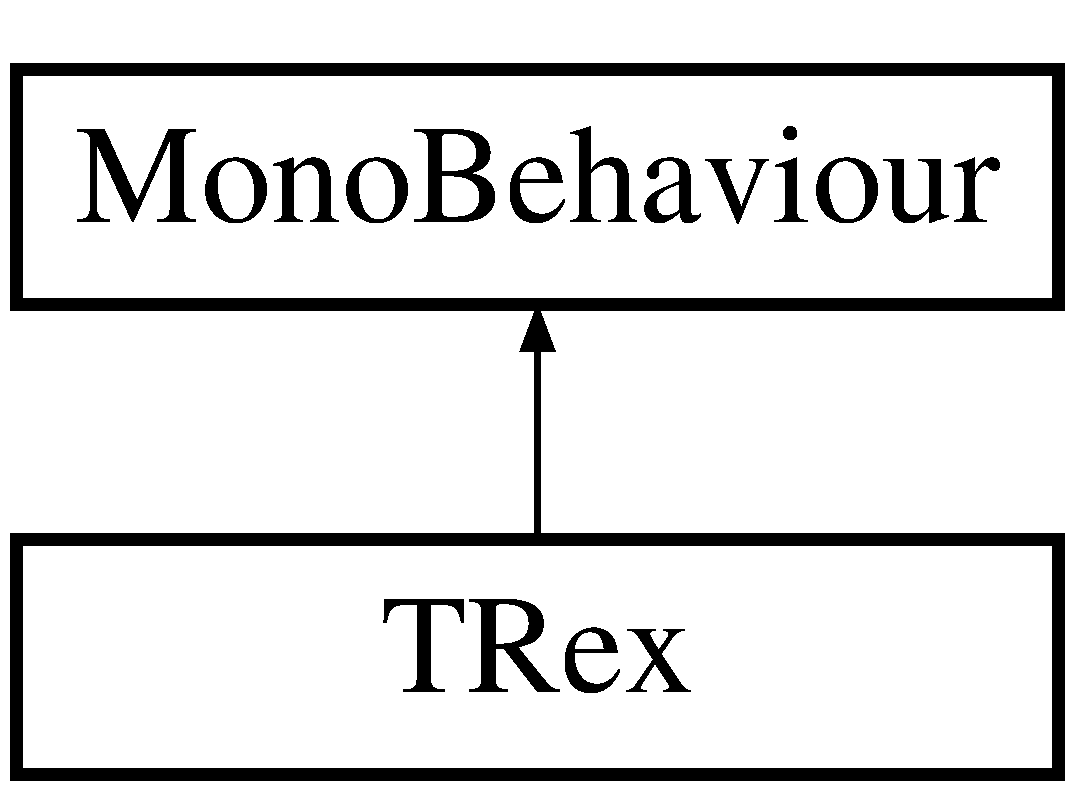
\includegraphics[height=2.000000cm]{class_t_rex}
\end{center}
\end{figure}
\subsection*{Public Attributes}
\begin{DoxyCompactItemize}
\item 
float \hyperlink{class_t_rex_ac2c1c5682d54b9a34e81a87db7232133}{move\+Speed}
\item 
float \hyperlink{class_t_rex_ad3cb47a8543233f79fa0506bf4ab9bf9}{jump\+Force}
\item 
bool \hyperlink{class_t_rex_a59fa915657244a351a19a6772868d10b}{is\+Grounded}
\item 
Layer\+Mask \hyperlink{class_t_rex_a91eb9e9165522f0f231a8e34f56d5919}{what\+Is\+Ground}
\end{DoxyCompactItemize}
\subsection*{Private Member Functions}
\begin{DoxyCompactItemize}
\item 
void \hyperlink{class_t_rex_ab9ca989e4ae071cad6a6766be74ff428}{Start} ()
\item 
void \hyperlink{class_t_rex_ab15426b15c8f9300d335aaeee5a7a7fc}{Update} ()
\item 
void \hyperlink{class_t_rex_a55c1bb4f0e4365269b1022cc9aa4ca8f}{Jump} ()
\begin{DoxyCompactList}\small\item\em $<$/\+Jump$>$ \end{DoxyCompactList}\end{DoxyCompactItemize}
\subsection*{Private Attributes}
\begin{DoxyCompactItemize}
\item 
Rigidbody2D \hyperlink{class_t_rex_afe1565632a661b2b0141b23ff2c26494}{t\+Rex\+Rigid\+Body}
\item 
Collider2D \hyperlink{class_t_rex_a40c401b1a7d0fd1eddd6947f42da7bb8}{my\+Collider}
\end{DoxyCompactItemize}


\subsection{Detailed Description}
$<$\+T\+Rex$>$ Kelas \hyperlink{class_t_rex}{T\+Rex} berfungsi untuk menangani input dari user dan mengeluarkan output ke layar berupa pergerakan dari \hyperlink{class_t_rex}{T\+Rex} $<$/\+Trex$>$ 

\subsection{Member Function Documentation}
\hypertarget{class_t_rex_a55c1bb4f0e4365269b1022cc9aa4ca8f}{}\label{class_t_rex_a55c1bb4f0e4365269b1022cc9aa4ca8f} 
\index{T\+Rex@{T\+Rex}!Jump@{Jump}}
\index{Jump@{Jump}!T\+Rex@{T\+Rex}}
\subsubsection{\texorpdfstring{Jump()}{Jump()}}
{\footnotesize\ttfamily void T\+Rex.\+Jump (\begin{DoxyParamCaption}{ }\end{DoxyParamCaption})\hspace{0.3cm}{\ttfamily [private]}}



$<$/\+Jump$>$ 

$<$/\+Jump$>$ Method jump berfungsi untuk menangani kasus jika \hyperlink{class_t_rex}{T\+Rex} ingin meloncat pada saat game sedang berjalan. \hypertarget{class_t_rex_ab9ca989e4ae071cad6a6766be74ff428}{}\label{class_t_rex_ab9ca989e4ae071cad6a6766be74ff428} 
\index{T\+Rex@{T\+Rex}!Start@{Start}}
\index{Start@{Start}!T\+Rex@{T\+Rex}}
\subsubsection{\texorpdfstring{Start()}{Start()}}
{\footnotesize\ttfamily void T\+Rex.\+Start (\begin{DoxyParamCaption}{ }\end{DoxyParamCaption})\hspace{0.3cm}{\ttfamily [private]}}

$<$\+Start$>$ Method start berfungsi untuk melakukan inisialisasi pertama pada saat game dimulai. $<$/\+Start$>$ \hypertarget{class_t_rex_ab15426b15c8f9300d335aaeee5a7a7fc}{}\label{class_t_rex_ab15426b15c8f9300d335aaeee5a7a7fc} 
\index{T\+Rex@{T\+Rex}!Update@{Update}}
\index{Update@{Update}!T\+Rex@{T\+Rex}}
\subsubsection{\texorpdfstring{Update()}{Update()}}
{\footnotesize\ttfamily void T\+Rex.\+Update (\begin{DoxyParamCaption}{ }\end{DoxyParamCaption})\hspace{0.3cm}{\ttfamily [private]}}

$<$\+Update$>$ Method update berfungsi untuk menangani kasus-\/kasus disaat terjadi perubahan frame pada saat game sedang berjalan. $<$/\+Update$>$ 

\subsection{Member Data Documentation}
\hypertarget{class_t_rex_a59fa915657244a351a19a6772868d10b}{}\label{class_t_rex_a59fa915657244a351a19a6772868d10b} 
\index{T\+Rex@{T\+Rex}!is\+Grounded@{is\+Grounded}}
\index{is\+Grounded@{is\+Grounded}!T\+Rex@{T\+Rex}}
\subsubsection{\texorpdfstring{is\+Grounded}{isGrounded}}
{\footnotesize\ttfamily bool T\+Rex.\+is\+Grounded}

$<$is\+Grounded$>$ Attribute is\+Grounded berfungsi untuk mencek apakah \hyperlink{class_t_rex}{T\+Rex} menempel dengan ground atau tidak. $<$/is\+Grounded$>$ \hypertarget{class_t_rex_ad3cb47a8543233f79fa0506bf4ab9bf9}{}\label{class_t_rex_ad3cb47a8543233f79fa0506bf4ab9bf9} 
\index{T\+Rex@{T\+Rex}!jump\+Force@{jump\+Force}}
\index{jump\+Force@{jump\+Force}!T\+Rex@{T\+Rex}}
\subsubsection{\texorpdfstring{jump\+Force}{jumpForce}}
{\footnotesize\ttfamily float T\+Rex.\+jump\+Force}

$<$jump\+Force$>$ Attribute jump\+Force berfungsi untuk mengatur kekuatan loncat \hyperlink{class_t_rex}{T\+Rex}. $<$/jump\+Force$>$ \hypertarget{class_t_rex_ac2c1c5682d54b9a34e81a87db7232133}{}\label{class_t_rex_ac2c1c5682d54b9a34e81a87db7232133} 
\index{T\+Rex@{T\+Rex}!move\+Speed@{move\+Speed}}
\index{move\+Speed@{move\+Speed}!T\+Rex@{T\+Rex}}
\subsubsection{\texorpdfstring{move\+Speed}{moveSpeed}}
{\footnotesize\ttfamily float T\+Rex.\+move\+Speed}

$<$move\+Speed$>$ Attribute move\+Speed berfungsi untuk mengatur kecepatan gerak \hyperlink{class_t_rex}{T\+Rex} $<$/move\+Speed$>$ \hypertarget{class_t_rex_a40c401b1a7d0fd1eddd6947f42da7bb8}{}\label{class_t_rex_a40c401b1a7d0fd1eddd6947f42da7bb8} 
\index{T\+Rex@{T\+Rex}!my\+Collider@{my\+Collider}}
\index{my\+Collider@{my\+Collider}!T\+Rex@{T\+Rex}}
\subsubsection{\texorpdfstring{my\+Collider}{myCollider}}
{\footnotesize\ttfamily Collider2D T\+Rex.\+my\+Collider\hspace{0.3cm}{\ttfamily [private]}}

$<$my\+Collider$>$ Attribute yang berfungsi untuk menangani kasus-\/kasus dimana \hyperlink{class_t_rex}{T\+Rex} akan menabrak suatu obstacle. $<$/my\+Collider$>$ \hypertarget{class_t_rex_afe1565632a661b2b0141b23ff2c26494}{}\label{class_t_rex_afe1565632a661b2b0141b23ff2c26494} 
\index{T\+Rex@{T\+Rex}!t\+Rex\+Rigid\+Body@{t\+Rex\+Rigid\+Body}}
\index{t\+Rex\+Rigid\+Body@{t\+Rex\+Rigid\+Body}!T\+Rex@{T\+Rex}}
\subsubsection{\texorpdfstring{t\+Rex\+Rigid\+Body}{tRexRigidBody}}
{\footnotesize\ttfamily Rigidbody2D T\+Rex.\+t\+Rex\+Rigid\+Body\hspace{0.3cm}{\ttfamily [private]}}

$<$trex\+Rigid\+Body$>$ Attribute trex\+Rigid\+Body berfungsi untuk membuat suatu object memiliki berat dan berpengaruh terhadap gravitasi. $<$/trex\+Rigid\+Body$>$ \hypertarget{class_t_rex_a91eb9e9165522f0f231a8e34f56d5919}{}\label{class_t_rex_a91eb9e9165522f0f231a8e34f56d5919} 
\index{T\+Rex@{T\+Rex}!what\+Is\+Ground@{what\+Is\+Ground}}
\index{what\+Is\+Ground@{what\+Is\+Ground}!T\+Rex@{T\+Rex}}
\subsubsection{\texorpdfstring{what\+Is\+Ground}{whatIsGround}}
{\footnotesize\ttfamily Layer\+Mask T\+Rex.\+what\+Is\+Ground}

$<$what\+Is\+Ground$>$ Attribute yang berisi layer yang berfungsi untuk memberikan informasi apakah \hyperlink{class_t_rex}{T\+Rex} berada di ground atau tidak yang berfungsi untuk menangani \hyperlink{class_t_rex}{T\+Rex} agar tidak dapat melakukan dua kali loncatan. $<$/what\+Is\+Ground$>$ 

The documentation for this class was generated from the following file\+:\begin{DoxyCompactItemize}
\item 
E\+:/\+Kuliah -\/ temporary/\+Semester 3/\+A\+D\+B\+O/\+Tugas Besar/\+T-\/\+Rex Final/assets/\+Scripts/T\+Rex.\+cs\end{DoxyCompactItemize}

%--- End generated contents ---

% Index
\backmatter
\newpage
\phantomsection
\clearemptydoublepage
\addcontentsline{toc}{chapter}{Index}
\printindex

\end{document}
